\chapter{前提知識}
本書で想定しているコンピュータのハードウェアやソフトウェアの
構成について解説する.

%==============================================================================
\section{コンピュータのハードウェア構成}
本書は,
コンピュータのハードウェア構成が\figref{hardBlock}のようになっている
ことを前提にしている.
複数のCPU(Central Processing Unit)がメモリを共有し,
また,全てのCPUは同じ機能を持ち優劣が無い.
このような方式を
\emph{SMP(対称型マルチプロセッシング:Symmetric Multiprocessing)}と呼ぶ.
メモリはCPUだけでなく,
I/Oコントローラ(\figref{hardBlock}ではアダプタやコントローラ)にも
共有される.

\begin{myfig}{btp}{ハードウエア構成}{hardBlock}
  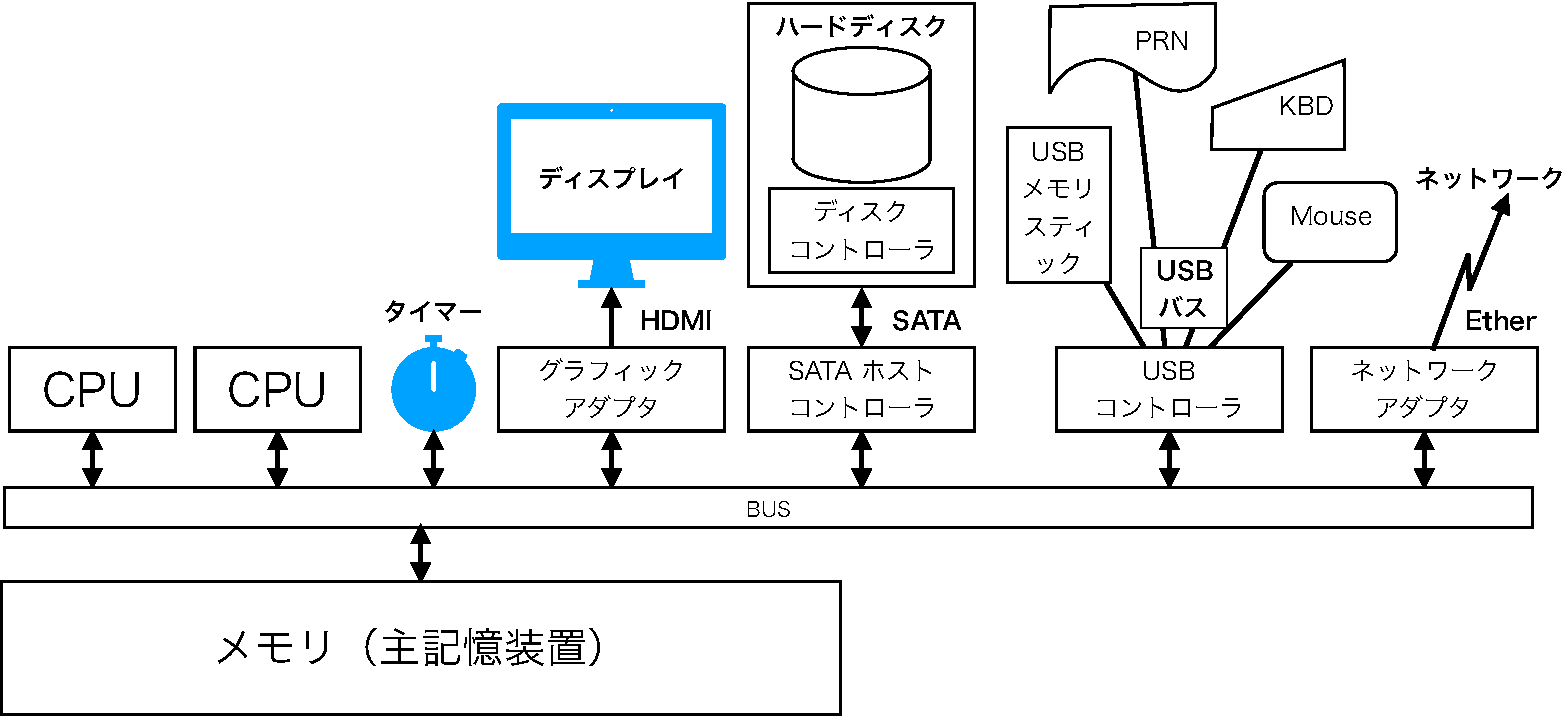
\includegraphics[scale=0.55]{Fig/hardBlock-crop.pdf}
\end{myfig}

\begin{enumerate}
\item CPU \\
  CPUはコンピュータの頭脳である.
  図はCPUが二つの構成になっているが,
  実際は一つの場合も,もっと多い場合もある.
\item メモリ(主記憶装置) \\
  プログラムやデータを記憶し,
  プログラム実行する際にCPUが直接使用する記憶装置である.
\item タイマー \\
  一定間隔で繰り返しCPUに割込みを発生するインターバルタイマーである.
\item グラフィックアダプタ \\
  ディスプレイを接続するためのアダプタである.
  表示内容を記憶するメモリを独自に持つ場合と,
  主記憶装置を使用する場合がある.
  最近のパーソナルコンピュータでは,
  グラフィックアダプタにGPU(Graphics Processing Unit)が組込まれている.
\item SATA ホストコントローラ \\
  SATA(Serial Advanced Technology Attachment)は,
  パーソナルコンピュータと二次記憶装置(ハードディスクやCD-ROM)を
  接続するためのインタフェース規格である.
  SATA ホストコントローラは次のような動作をする.
  \begin{enumerate}
  \item CPUがSATAホストコントローラにコマンドを書き込む.
    コマンドは,
    「読み/書き」,「セクタアドレス」,「セクタ数」,「メモリアドレス」
    を含んだものである.
  \item SATAホストコントローラは,
    ディスクコントローラと通信しハードディスクにコマンドを渡す.
  \item ハードディスクの読み・書きが可能になったら,
    ホストコントローラはハードディスクとメモリの間でデータ転送を行う.
    このようなCPUを介さないデータ転送のことを,
    \emph{DMA(Direct Memory Access)}\label{dma}と呼ぶ.
  \item SATAホストコントローラはCPUに割込み信号を送り,
    データの転送が完了したことを知らせる.(\emph{I/O完了割込み})
  \end{enumerate}
  CPUは,
  SATAホストコントローラにコマンドを送ってから割込みが発生するまでの間,
  他の仕事をすることができる.
  ハードディスクの操作(I/O操作)とCPUの計算は並列実行される.
\item USBホストコントローラ \\
  USB(Universal Serial Bus)は,
  パーソナルコンピュータと周辺装置を手軽に接続できるインタフェースである.
  USBメモリスティックやプリンタ,キーボード,マウス等,多くの周辺装置が
  USBを通して接続できる.
  USBコントローラもSATAホストコントローラのようにDMA機能を備えている.
\item ネットワークアダプタ \\
  パーソナルコンピュータのネットワークアダプタは,
  GbE(Gigabit Ethernet)規格のものが普及している.
  これもSATAホストコントローラのようにDMA機能を備えている.
\item BUS(バス) \\
  パーソナルコンピュータのハードウェアを構成する装置の間で
  データをやり取りするための配線である.
  CPUだけでなくDMAを使用するコントローラや
  アダプタが大量のデータ転送を行うので,
  バスのデータ転送能力がパーソナルコンピュータの性能向上のボトルネックになる.

  そのため後で説明するように,実際の物理的な接続は\figref{hardBlock}とは
  かなり異なった構成になっている.
  しかし,オペレーティングシステムが意識しなければならない論理的な
  接続は\figref{hardBlock}のものである.
\end{enumerate}

%==============================================================================
\section{CPUの構成}
本書では、CPUは\figref{cpuBlock}の部品で構成されると考える.
\figref{hardBlock}に示したように,CPUはBUSを通して他の装置と接続される.
CPUは,一つの機械語命令の実行が終わり次の命令の実行を開始する前に,
他の装置から割込みを受け付けることができる\footnote{
  例外的に,メモリ管理に関する一部の割込は機械語命令の途中で発生する.}.

\begin{myfig}{btp}{CPUの構成}{cpuBlock}
  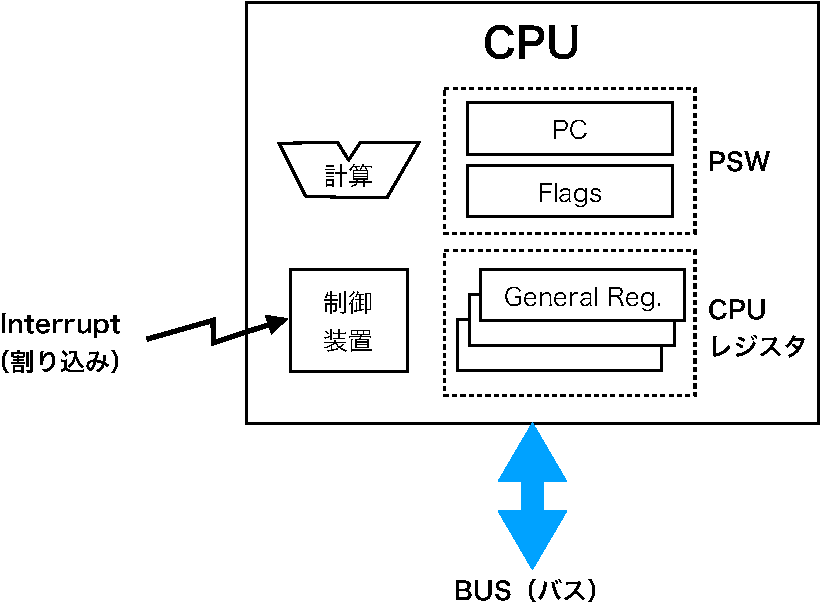
\includegraphics[scale=0.66]{Fig/cpuBlock-crop.pdf}
\end{myfig}

\begin{enumerate}
\item \emph{PSW(Program Status Word)} \\
  PSWは,PC(Program Counter)とFlags(フラグ)から構成されるものとする.
  PCはCPUが実行中のプログラムの命令アドレスを保持するカウンタである.
  Flagsには計算の結果によって変化するビットの他に,
  割込み許可/不許可を表現するビット,
  実行モード(ユーザモード/カーネルモード)を表現するビット等が含まれる.
\item \emph{CPUレジスタ} \\
  計算に使用するCPUの汎用レジスタのことである.
  TeCではG0,G1,G2,SPのこと,
  情報処理技術者試験のCOMETではGR0,GR1,GR2,GR3,GR4のことである.
\end{enumerate}

PSWとCPUレジスタは,
機械語命令を実行する度に値が変化・確定しプログラムが意識している\footnote{
  一方でCPU内部にはプログラムから見えないレジスタもある.
}ので,CPUを仮想化し,実行するプロセスを切換える際に保存・復旧の対象となる.

%==============================================================================
\section{最近のコンピュータの実際の構成}
Intel社のCPUを使用したデスクトップ・パーソナルコンピュータと
サーバコンピュータの構成を説明する.
バスがボトルネックにならないように,
CPUとメモリが直接に接続してある.

\subsection{デスクトップ・パーソナルコンピュータ}
\figref{intelDesktop}はIntel社のCPUを使用した
近年のデスクトップ・パーソナルコンピュータの構成を表している.
Intel社の用語では,これまで「CPU」と呼んでいたものを
「\emph{Core(コア)}」と呼ぶ.
「CPU」は複数のコアを含んだLSIのことを指している.
デスクトップ用のCPUには1〜4個のコアが集積されている.

\begin{myfig}{btp}{デスクトップPCの構成}{intelDesktop}
  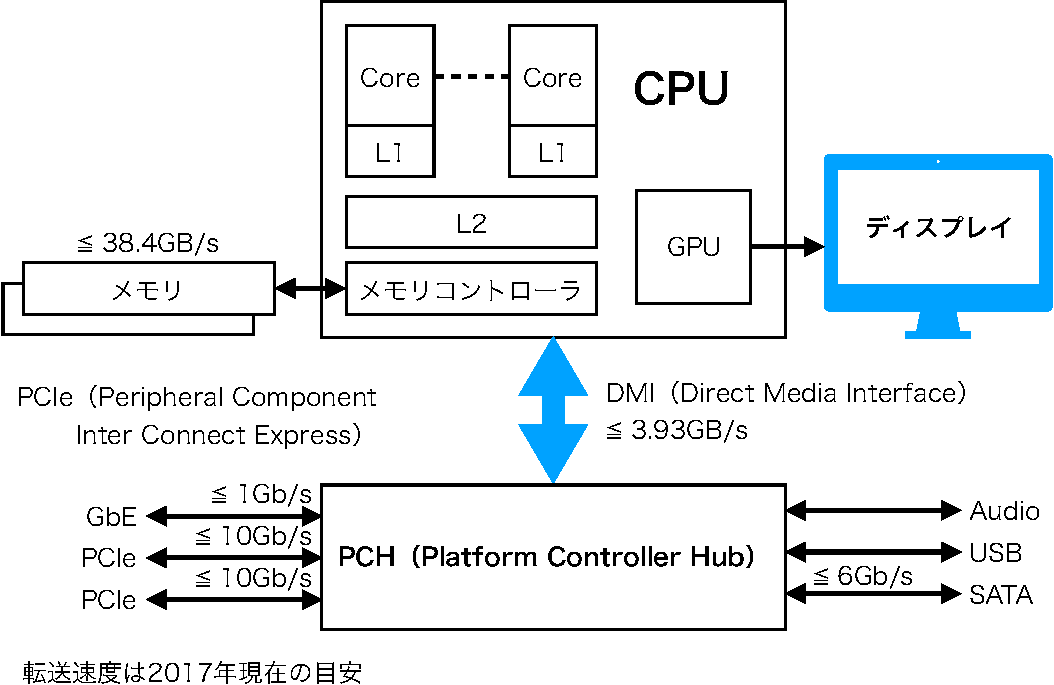
\includegraphics[scale=0.66]{Fig/intelDesktop-crop.pdf}
\end{myfig}

コアに隣接しているL1はレベル1キャッシュ(Level 1 cache)を表している.
L2は複数のコアにシェアされるレベル2キャッシュ(Level 2 cache)を表している.
メモリとのデータ転送量が多いCoreとGPUがCPUに集積され,
I/O装置のホストコントローラやアダプタはPCHに集積されている.
CPUとPCHはDMIと呼ばれる専用のインタフェースを用いて接続される.

\subsection{サーバコンピュータ}
より強力な処理能力が必要なサーバ用コンピュータでは,
\figref{intelServer}のように多くのコアを内蔵するCPUを複数個使用する.
現在(2017年秋)最新の Intel Xeon Processor Scalable Family の場合,
CPU同士はUPIと呼ばれる高速な専用インタフェースで接続される.
最大の構成は,28コアのCPUを8個使用し合計224コアのものである.
PCHもサーバ用のものは,より多くのストレージやネットワークを接続できる.

\begin{myfig}{btp}{サーバPCの構成}{intelServer}
  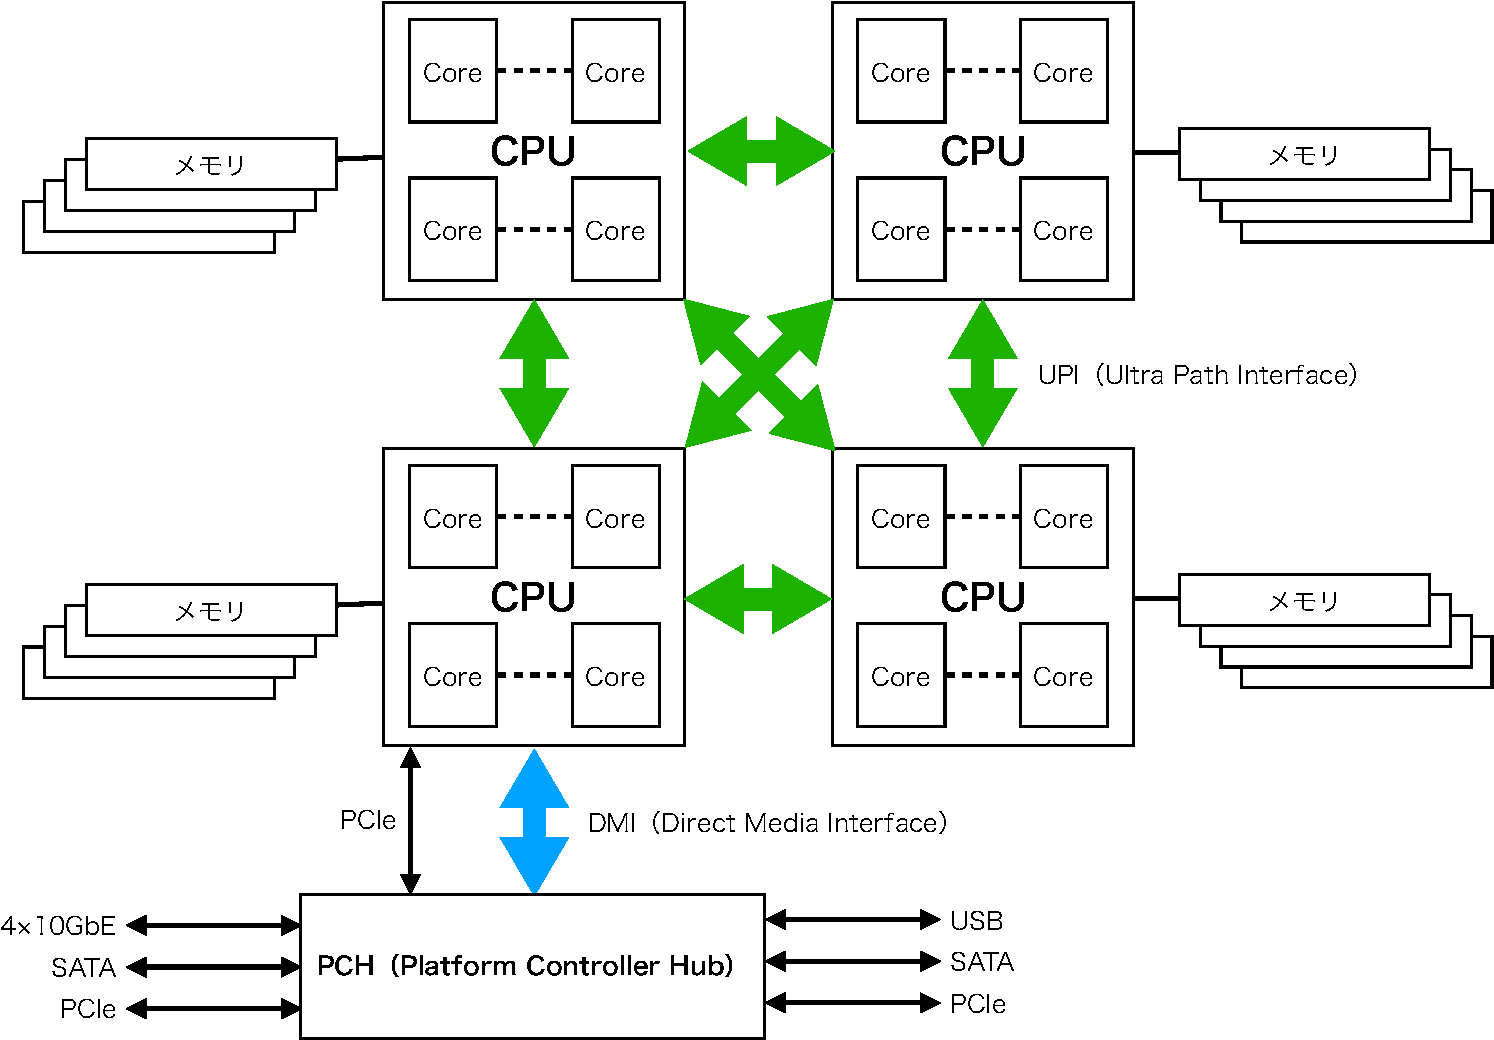
\includegraphics[scale=0.6]{Fig/intelServer-crop.pdf}
\end{myfig}

%==============================================================================
\section{割込み}
\label{interruptSource}
通常,コンピュータはユーザ・プロセスを実行し目的の仕事をしている.
何かイベントが発生すると割込みによりCPUに通知される.
CPUはカーネルモードに切り替わり割込みハンドラに制御を移す.
CPUがユーザ・プロセスの実行からカーネルの実行に移行するのは,
\emph{割込みが発生した時だけ}である.

カーネルへ実行を移すには割込みを発生する以外に方法がない.
割込みが発生する原因には以下のものがある.
システムコール以外はユーザ・プロセスが意図しない間に発生する.

\begin{enumerate}
\item I/O完了・タイマー \\
  ホストコントローラやネットワークアダプタ,タイマー等のハードウェアが,
  コマンドの実行完了等をCPUに知らせるために発生する.
\item システムコール \\
  ユーザ・プロセスは,
  割込みを発生する特殊な機械語命令である\emph{SVC(Supervisor Call)}命令
  \footnote{
    CPUによってはTRAP命令,INT命令と呼ばれることもある.
  }
  を用いて
  システムコールを発行する.
  カーネルはSVC命令実行時のCPUレジスタの値などから
  システムコールの種類やパラメータを知ることができる.
\item 保護違反 \\
  ユーザ・プロセスが,
  ユーザ・モードでは実行が許可されない命令を実行したり,
  アクセスが許可されないメモリ領域をアクセスした場合に発生する.
\item ソフトウェアのエラー \\
  ユーザ・プロセス実行中に計算でオーバーフローが発生した場合等に発生する.
\item ハードウェアのエラー \\
  ハードウェアの故障や電源の異常を検知した時に発生する.
\end{enumerate}

%==============================================================================
\section{オペレーティングシステムの構造}
\figref{osOrganization}にオペレーティングシステムの構造を示す.
カーネルは\figref{osOrganization}中央部分のソフトウェアである.
ユーザプロセスはユーザモードで,
カーネルはカーネルモードで実行される.

\begin{myfig}{btp}{オペレーティングシステムの構造}{osOrganization}
  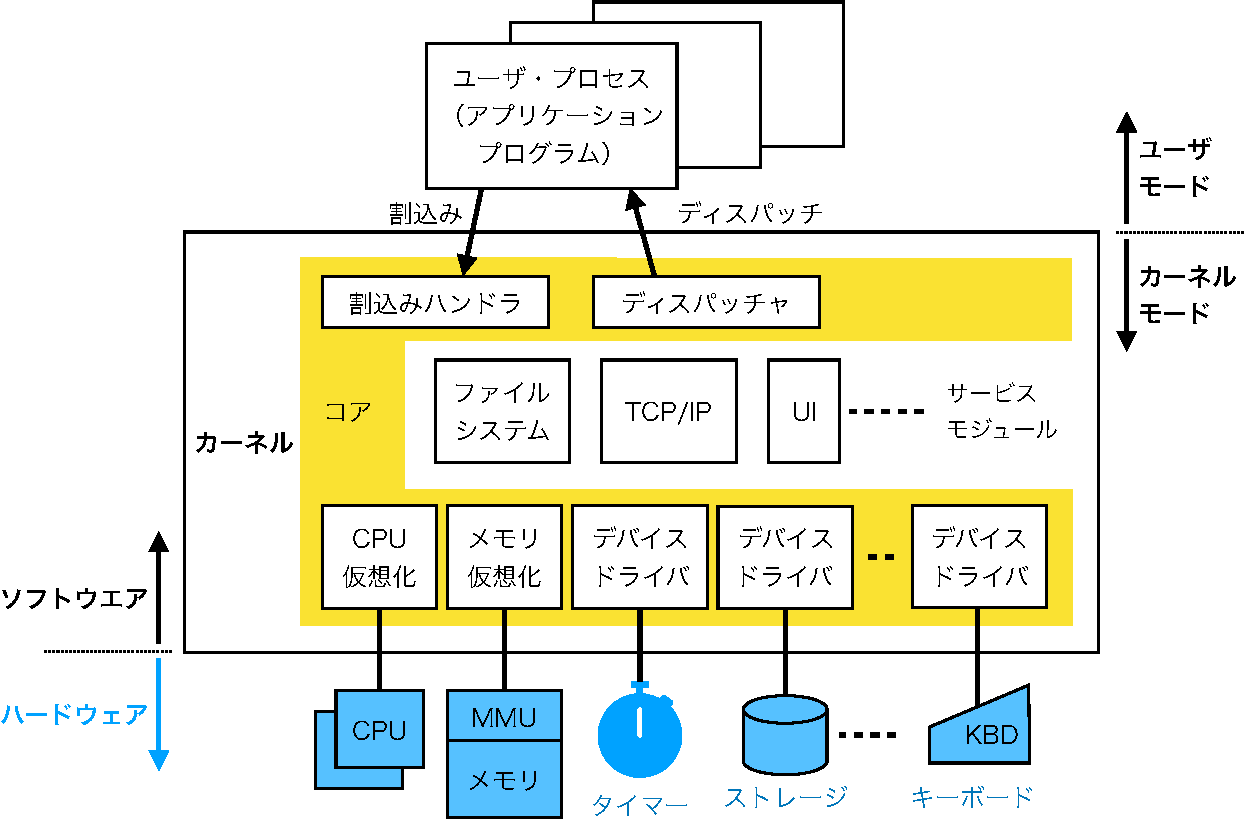
\includegraphics[scale=0.66]{Fig/osOrganization-crop.pdf}
\end{myfig}

\subsection{カーネルの構成}
カーネルは以下のモジュールから構成される.

\begin{enumerate}
\item \emph{割込みハンドラ} \\
  割込みが発生した時に自動的に実行される割込み処理ルーチンである.
  割込みが発生した原因を判断し,必要なモジュールを呼び出す.
  例えば,タイマーからの割込みならタイマーのデバイスドライバを呼び出す.
\item \emph{ディスパッチャ} \\
  カーネルの処理が終了した時,
  実行可能なプロセスの中から一つを選んで実行を再開する.
\item \emph{コア} \\
  コアは,資源の仮想化を行うために,必ずカーネルモードで実行する必要がある.
\item \emph{サービスモジュール} \\
  サービスモジュールは,
  ハードウェアを抽象化した便利なコンピュータを
  ユーザ・プロセスに提供するためのプログラムである.
\item \emph{デバイスドライバ} \\
  ハードウェアを制御するソフトウェアである.
  ハードウェアの差異を吸収し抽象化したインタフェースをカーネルに提供する.
  例えば,同じキーボードでも,
  PS/2,USBなどの接続方式や機種などにより制御方法は大幅に異なる.
  一方でカーネルが必要としているAPIは一定である.
  デバイスドライバがキーボードの機種ごとの差異を吸収する.
\end{enumerate}

割込みが発生するとカーネル・モードに切り換わり割込みハンドラに制御が移る.
その後,カーネル内では以下の手順で処理がされる.

\begin{enumerate}
\item 割込みハンドラは後でプロセスの実行を再開できるように,
  プロセスのCPUの状態(\emph{コンテキスト}:PSW,CPUレジスタ)を保存する.
\item 割込みハンドラは割込み原因を調べ,
  原因に応じたカーネル内のサービスモジュールやデバイスドライバに制御を渡す.
  例えばファイル操作のシステムコールならファイルシステムへ制御を渡す.
\item サービスモジュールやデバイスドライバの処理が終了したら
  ディスパッチャに制御が渡される.
  ディスパッチャは実行可能なプロセスの一つを選び,
  コンテキストを復旧しプロセスの実行を再開する.
\end{enumerate}

\subsection{プロセスの構造}
\figref{osOrganization}のユーザ・プロセス部分を詳しく描いたものを
\figref{procOrganization}に示す.

\begin{myfig}{btp}{プロセスの構造}{procOrganization}
  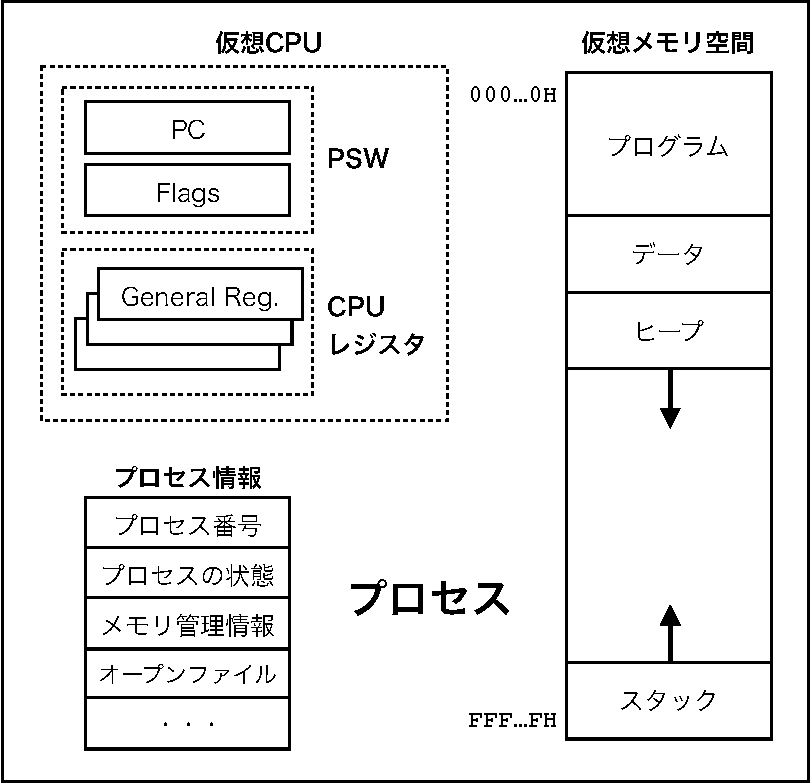
\includegraphics[scale=0.66]{Fig/procOrganization-crop.pdf}
\end{myfig}

\begin{enumerate}
\item \emph{仮想CPU} \\
  CPUを仮想化し,
  プロセス毎にCPUが存在するように見せることで,
  マルチプログラミングを可能にする.
  プロセスがCPUを使用する時間を区切り,
  次々に切替える時分割多重によりCPUの仮想化は達成される.

  他のプロセスがCPUを使用している間に,
  プロセスのコンテキストを保存する領域を仮想CPUと呼ぶことにする.
  ハードウェアの実CPUに対応してPSWとCPUレジスタの保存先が必要である.
  前の節で説明したように,
  プロセスからカーネルに制御が移る時にプロセスのコンテキストを保存する.
  プロセス実行時にはコンテキストが実CPUにロードされる.
\item \emph{仮想メモリ空間} \\
  メモリを仮想化しプロセス毎に専用のメモリ空間が存在するように見せかける.
  実現方法は第\ref{memoryManagement}部「メモリ管理」で詳しく学ぶ.
  仮想メモリ空間は次の部分から構成される.
  \begin{enumerate}
  \item プログラム \\
    機械語プログラムがここに配置される.
    C言語で記述されたプログラムの場合,
    関数の実行文(式文,if文,for文,while文など)が
    翻訳された機械語が該当する.
  \item データ \\
    プログラムの変数部分がここに配置される.
    C言語ではグローバル変数が該当する.
  \item ヒープ \\
    プログラム実行時に動的に拡大される領域である.
    C言語の\|malloc()|関数はヒープに新しい領域を確保する.
    \|malloc()|関数が使用される度にヒープ領域は後ろに向かって拡大する.
  \item スタック \\
    プログラム実行時にメモリ空間の最後から前に向かって伸びる領域である.
    サブルーチン・コール時に戻りアドレスを保存したり,
    C言語のローカル変数や関数引数を置いたりする.
  \end{enumerate}
\item \emph{プロセス情報} \\
  名前にあたる「プロセス番号」,
  実行中/実行可能/待ちのどの状態なのか表す「プロセスの状態」,
  使用しているメモリの大きさ等を表す「メモリ管理情報」,
  CPUを使用した時間を表す「CPU時間」等の情報のことである\footnote{
    これらはUNIXのpsコマンドで表示することができる.}.
  その他に,プロセスが現在オープンしているファイルに関する情報や,
  親プロセス,子プロセス,シグナルハンドラの登録状況,
  プロセスの優先度など,様々な情報がここに記録される.
\end{enumerate}

%==============================================================================
\section{カーネルの構成方式}
カーネルが動作不良を起こすと
実行中の全てのユーザ・プロセスを巻き込んでシステムが停止するので,
カーネルには非常に高い信頼性が要求される.
しかし,カーネルは非常に大きなプログラムになりがちであり\footnote{
  Linux や Windows のカーネルのソースコードは500万行にもなる\cite{lines}.},
高い信頼性を確保するにはカーネルの構成方法に工夫が必要である.
%一方でカーネルの処理が重くなると全てのユーザ・プロセスに影響するので,
%効率も犠牲にすることはできない.

\subsection{単層カーネル(モノリシック・カーネル)}
最も一般的な構成方法である.
\figref{osOrganization}のカーネルは単層カーネルの例になっている.
カーネル内の全てのモジュールがリンクされ,一つのプログラムになる.
カーネル内でモジュールの呼び出しはCALL機械語命令を用いて行うので効率が良い.
しかし,モジュール同士が密にリンクされているので,
モジュール間で情報の隠蔽がし難くバグが入りやすい.
また,全てのモジュールがカーネル・モードで実行されるので,
一つのモジュールのバグが致命的な結果を引き起こす.
LinuxやFreeBSDは,この方式のカーネルを持つ.

\subsection{マイクロカーネル(micro-kernel)}
\figref{osOrganization}の「コア」からデバイスドライバを取り除き\footnote{
  タイマーのデバイスドライバはCPUの仮想化に必要なので,
  マイクロカーネルに残す.},
カーネル(マイクロカーネル)とし構成する方式である.
\figref{microkernel}にマイクロカーネル方式の概要を示す.
カーネル・モードで実行されるのはマイクロカーネルだけである.

\begin{myfig}{btp}{マイクロカーネル方式}{microkernel}
  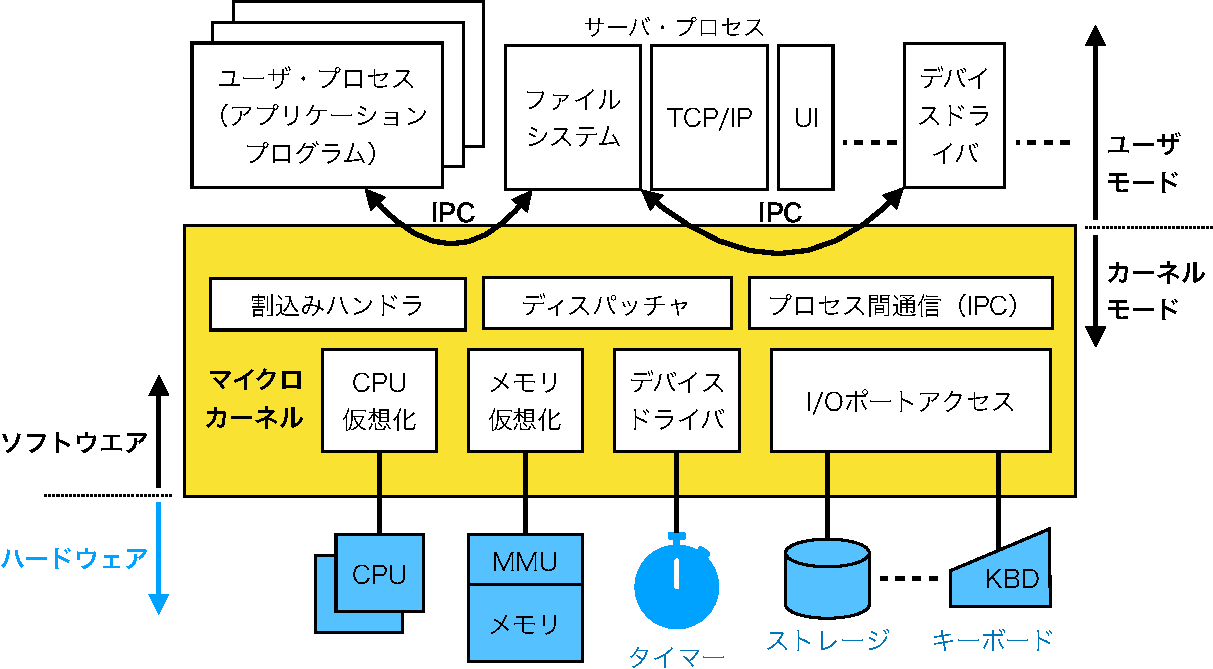
\includegraphics[scale=0.66]{Fig/microkernel-crop.pdf}
\end{myfig}

サービスモジュールはカーネルから独立したサーバ・プロセスとし,
権限の低いユーザ・モードで実行される.
ユーザ・プロセスは,マイクロカーネルが提供する
\emph{IPC(プロセス間通信:Inter-Process Communication)}を用いて,
サーバ・プロセスにサービスを要求する.
サーバ・プロセス同士,サーバ・プロセスとデバイスドライバ・プロセスも
IPCを用いて通信する.

デバイスドライバはI/Oポートにアクセスするのでカーネル・モードで
実行される必要があると考えられるが,
I/Oポートへのアクセスをマイクロカーネルのシステムコールに置換えることで,
デバイスドライバもユーザ・プロセスとして実装することが可能である.
この場合は,アクセスしても良いI/Oアドレスの範囲内かどうか,
マイクロカーネルがチェックすることが可能である.

マイクロカーネル方式は,
サービスモジュールやデバイスドライバが権限の低いプロセスとして実行されるので,
これらのバグでシステム全体が停止する危険性が低い。
また,
サービスモジュールやデバイスドライバ毎に独立したプログラムになり
モジュール化が徹底しやすいので,
巨大な単一プログラムであるモノリシックカーネルと比較してバグが発生しにくい.
信頼性の高いオペレーティングシステムを構成するために有利である.
しかし,IPCとプロセス切り換えのオーバヘッドが大きいため性能が低くなる.
\emph{多くの場合,信頼性と性能はトレードオフの関係にある.}

%==============================================================================
\section{もう一つの仮想マシン}
\ref{osRole}で述べたように,
オペレーティングシステムは抽象化され便利な拡張マシン(仮想マシン)を,
必要な数だけ提供する.
ここで述べた仮想マシンは,単一のユーザ・プロセスを実行する環境のことである.
同じ「仮想マシン」と言う用語が,
オペレーティングシステムを実行することが可能な,
よりハードウェアを忠実に再現した仮想マシンを指す場合もある.
ここでは,
一台のコンピュータ上で複数のオペレーティングシステムを実行可能な,
もう一つの仮想マシンについて紹介する.

\subsection{Type 2 ハイパーバイザ}
例えば,
Macを使用している人がWindowsでしか動作しないアプリケーションを使用する
場合を想像してしてみる\footnote{
  徳山高専情報電子工学科のパソコン室では,
  WindowsやLinuxでしか動作しないXilinx ISE WebPACKをMacで使用している.}.
予めMacのハードディスクにmacOSとは別にWindowsもインストールしておき,
電源投入時にmacOSとWindowsを選んでブートする方法もあるが,
オペレーティングシステムを切換える度にコンピュータを再起動するのは不便である.
また,macOSのアプリケーションとWindowsのアプリケーションを同時に実行したい
場合もある.

そこで,\figref{type2Hypervisor}に示す
「Type 2 ハイパーバイザ(Type 2 Hypervisor)」を用いた仮想化が用いられる.
ハイパーバイザは
\emph{ホスト・オペレーティングシステム}の一つのユーザプロセスとして実行され,
コンピュータ一台の機能をエミュレーションする.
ハイパーバイザがエミュレーションするコンピュータの中で,
\emph{ゲスト・オペレーティングシステム}が稼働する.
エミュレーションはソフトウェアだけで完全に行うのではなく\footnote{
  完全にソフトウェアで行う場合もある.},
ハードウェアの支援を受けて行うので高速に行うことができる\cite{virtualization}.
Type 2 ハイパーバイザとして有名は製品は,
VMware Workstation,
VMware Fusion,
VirtualBox\footnote{
  徳山高専情報電子工学科のパソコン室では
  macOS上のVirtualBoxでWindowsを動作させている.
  %このWindowsの中でXlinix ISE WebPACKが使用できる.
}等である.

\begin{myfig}{btp}{Type 2 ハイパーバイザ}{type2Hypervisor}
  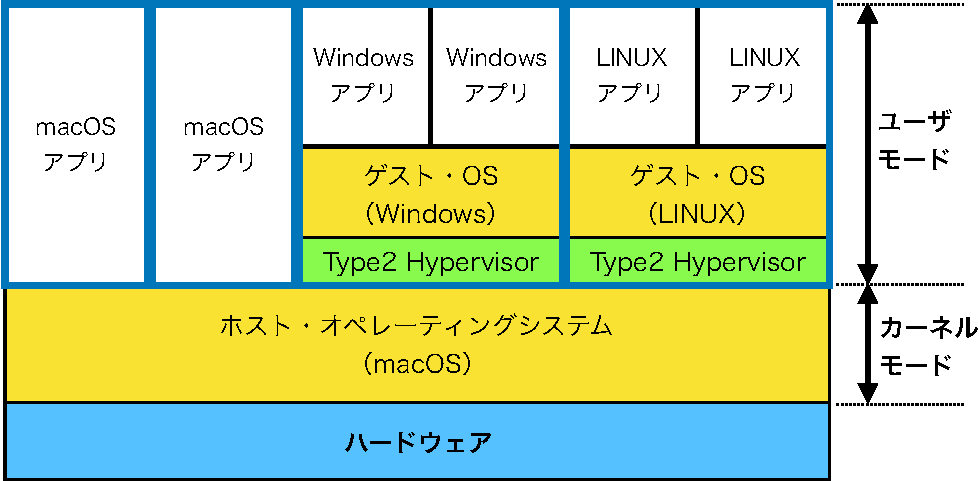
\includegraphics[scale=0.66]{Fig/type2Hypervisor-crop.pdf}
\end{myfig}

\subsection{Type 1 ハイパーバイザ}
メインフレーム上で1960年代から使用されている方式である.
現在ではPCサーバの仮想化にも使用されている.
Type 1 ハイパーバイザはホスト・オペレーティングシステム無しに
ハードウェア上で直接実行される.
Type 1 ハイパーバイザとして有名な製品は,
IBM z/VM,
VMware vSphere,
Xen,
Hyper-V等である.

サーバ向けの製品が主流であり,
例えば VMware vSphere は
実行中のゲストを他の物理サーバに移動する等,
非常に高度な機能を持っており\cite{vsphere},
一台のサーバ上に効率よく多数の仮想マシンを動かすことができる.
徳山高専情報電子工学科のパソコン室でも,
2台のサーバ上に50台の仮想デスクトップマシンを動かしていたことがある.

\begin{myfig}{btp}{Type 1 ハイパーバイザ}{type1Hypervisor}
  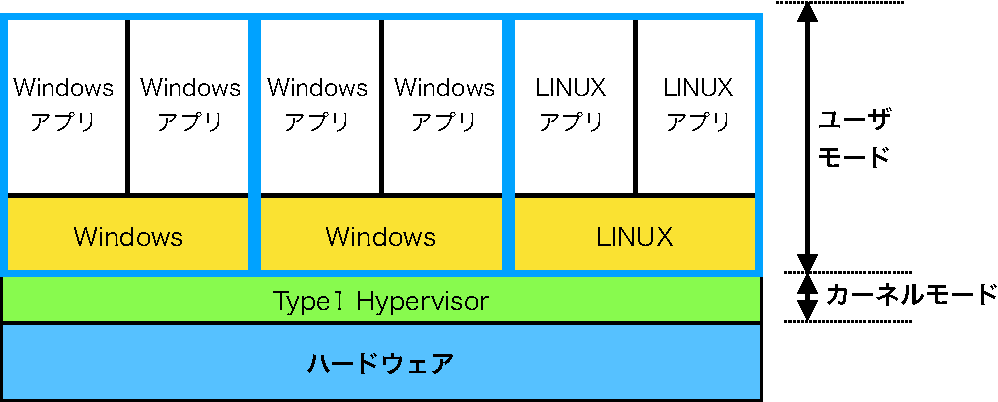
\includegraphics[scale=0.66]{Fig/type1Hypervisor-crop.pdf}
\end{myfig}

\subsection{仮想アプライアンス}
ゲスト・オペレーティングシステムとアプリケーションまでインストールし,
すぐに使用できる状態で配布される仮想マシンである.
例えば,メールフィルタソフトをインストールした仮想マシンを
入手しハイパーバイザで実行するだけで,
すぐにメールフィルタリングが開始できる.

同じ手法で,
すぐに使用できるパーソナルコンピュータ用の
デスクトップ・オペレーティングシステムが配布されている場合もある.
Linux の一種であるUbuntuの場合,
VirtualBoxで実行できるディスクイメージがダウンロードできる\cite{ubuntu}.
仮想アプライアンスは,
ソフトウェアの新しい流通手法である.

%==============================================================================
\section{実装例}
本書では,
TaC(Tokuyama Advanced educational Computer)と,
TaCのオペレーティングシステムTacOSを実装例として参照する.
第\ref{TacAndTacOS}章でTaCとTacOSの概要を紹介する.
TaCは,学生が限られた時間で仕組みを理解できるように設計された,
単純で小さな16ビットパーソナルコンピュータである.

%==============================================================================
\section{まとめ}
本書は\emph{SMP(対称型マルチプロセッシング:Symmetric Multiprocessing)}の
コンピュータを前提にしている.
CPUは\emph{PSW(Program Status Word)}と\emph{CPUレジスタ}を含んでいる.
最近のIntel社のCPUでは,従来のCPUを\emph{Core(コア)},
複数のコアを含んだLSIのことをCPUと呼ぶ.
SMPでは複数のCPU(コア)がメモリを共有する.
更に,ホストコントローラやアダプタも
\emph{DMA(Direct Memory Access)}方式によりメモリを共有する.

オペレーティングシステムのカーネルは,
割込みハンドラ,ディスパッチャ,サービスモジュール,
デバイスドライバ等から構成される.
ユーザ・プロセスからカーネルへの切換え原因は\emph{割込み}だけである.
ユーザ・プロセス毎に\emph{仮想CPU},\emph{仮想メモリ空間},管理情報等を
持っている.

カーネルの構成方式には,
\emph{単層カーネル(モノリシック・カーネル)}方式と
\emph{マイクロカーネル(micro-kernel)}方式の二種類があった.
マイクロカーネル方式ではサービスモジュールをサーバ・プロセスとし,
\emph{IPC(プロセス間通信)}を用いてサービスを要求する.
サービスモジュール間の独立性が高くなり高信頼性のシステムを構成可能であるが,
IPCはオーバーヘッドが大きい.
信頼性と性能はトレードオフの関係にある.

Type1,Type2ハイパバイザは,
PCのハードウェア全体をエミュレーションする仮想マシンを提供する.
この仮想マシンの上で,WindowsやLinux等のオペレーティングシステムを
実行することができる.

%==============================================================================
\section*{練習問題}
\begin{enumerate}
  \renewcommand{\labelenumi}{\ttfamily\arabic{chapter}.\arabic{enumi}}
  \setlength{\leftskip}{1em}
\item 次の言葉の意味を説明しなさい.
  \begin{enumerate}
    \item CPU
    \item ホストコントローラ
    \item バス
    \item DMA
    \item SMP(対象型マルチプロセッシング)
    \item PSW
    \item CPUレジスタ
    \item 割込み
    \item SVC命令
    \item ディスパッチャ
    \item サービスモジュール
    \item デバイスドライバ
    \item カーネルのコア
    \item コンテキスト
    \item 仮想CPU
    \item 仮想メモリ空間
    \item 単層カーネル(モノリシック・カーネル)
    \item マイクロカーネル
    \item IPC(プロセス間通信)
    \item Type 1 ハイパーバイザ
    \item Type 2 ハイパーバイザ
  \end{enumerate}
\item 自分がいつも使用しているパーソナルコンピュータの
  ハードウェア構成を調べなさい.
  \begin{enumerate}
    \item CPUの種類(名称,メーカ,クロック,コア数(CPU数))
    \item メモリの大きさ
    \item 二次記憶装置(ストレージ)の種類(ハードディスク?,SSD?)
    \item 二次記憶装置(ストレージ)の大きさ
    \item グラフィックアダプタの種類
    \item キーボードやマウスの接続方式(USB?,Bluetooth?)
  \end{enumerate}
\end{enumerate}
